% ===================================================================
% SECTION 3: METHODOLOGY
% ===================================================================
\section{Methodology}

% --- Subsection 3.1: Algorithms ---
\subsection{Algorithms}

% --- Slide 1 ---
\begin{frame}
    \frametitle{Scalability Limits of Traditional \& Commercial Solvers}

    \begin{columns}[T]
        
        % --- LEFT COLUMN: Traditional Exact Algorithms ---
        \begin{column}{0.5\textwidth}
            \begin{block}{1. Space Complexity}
                \begin{figure}
                    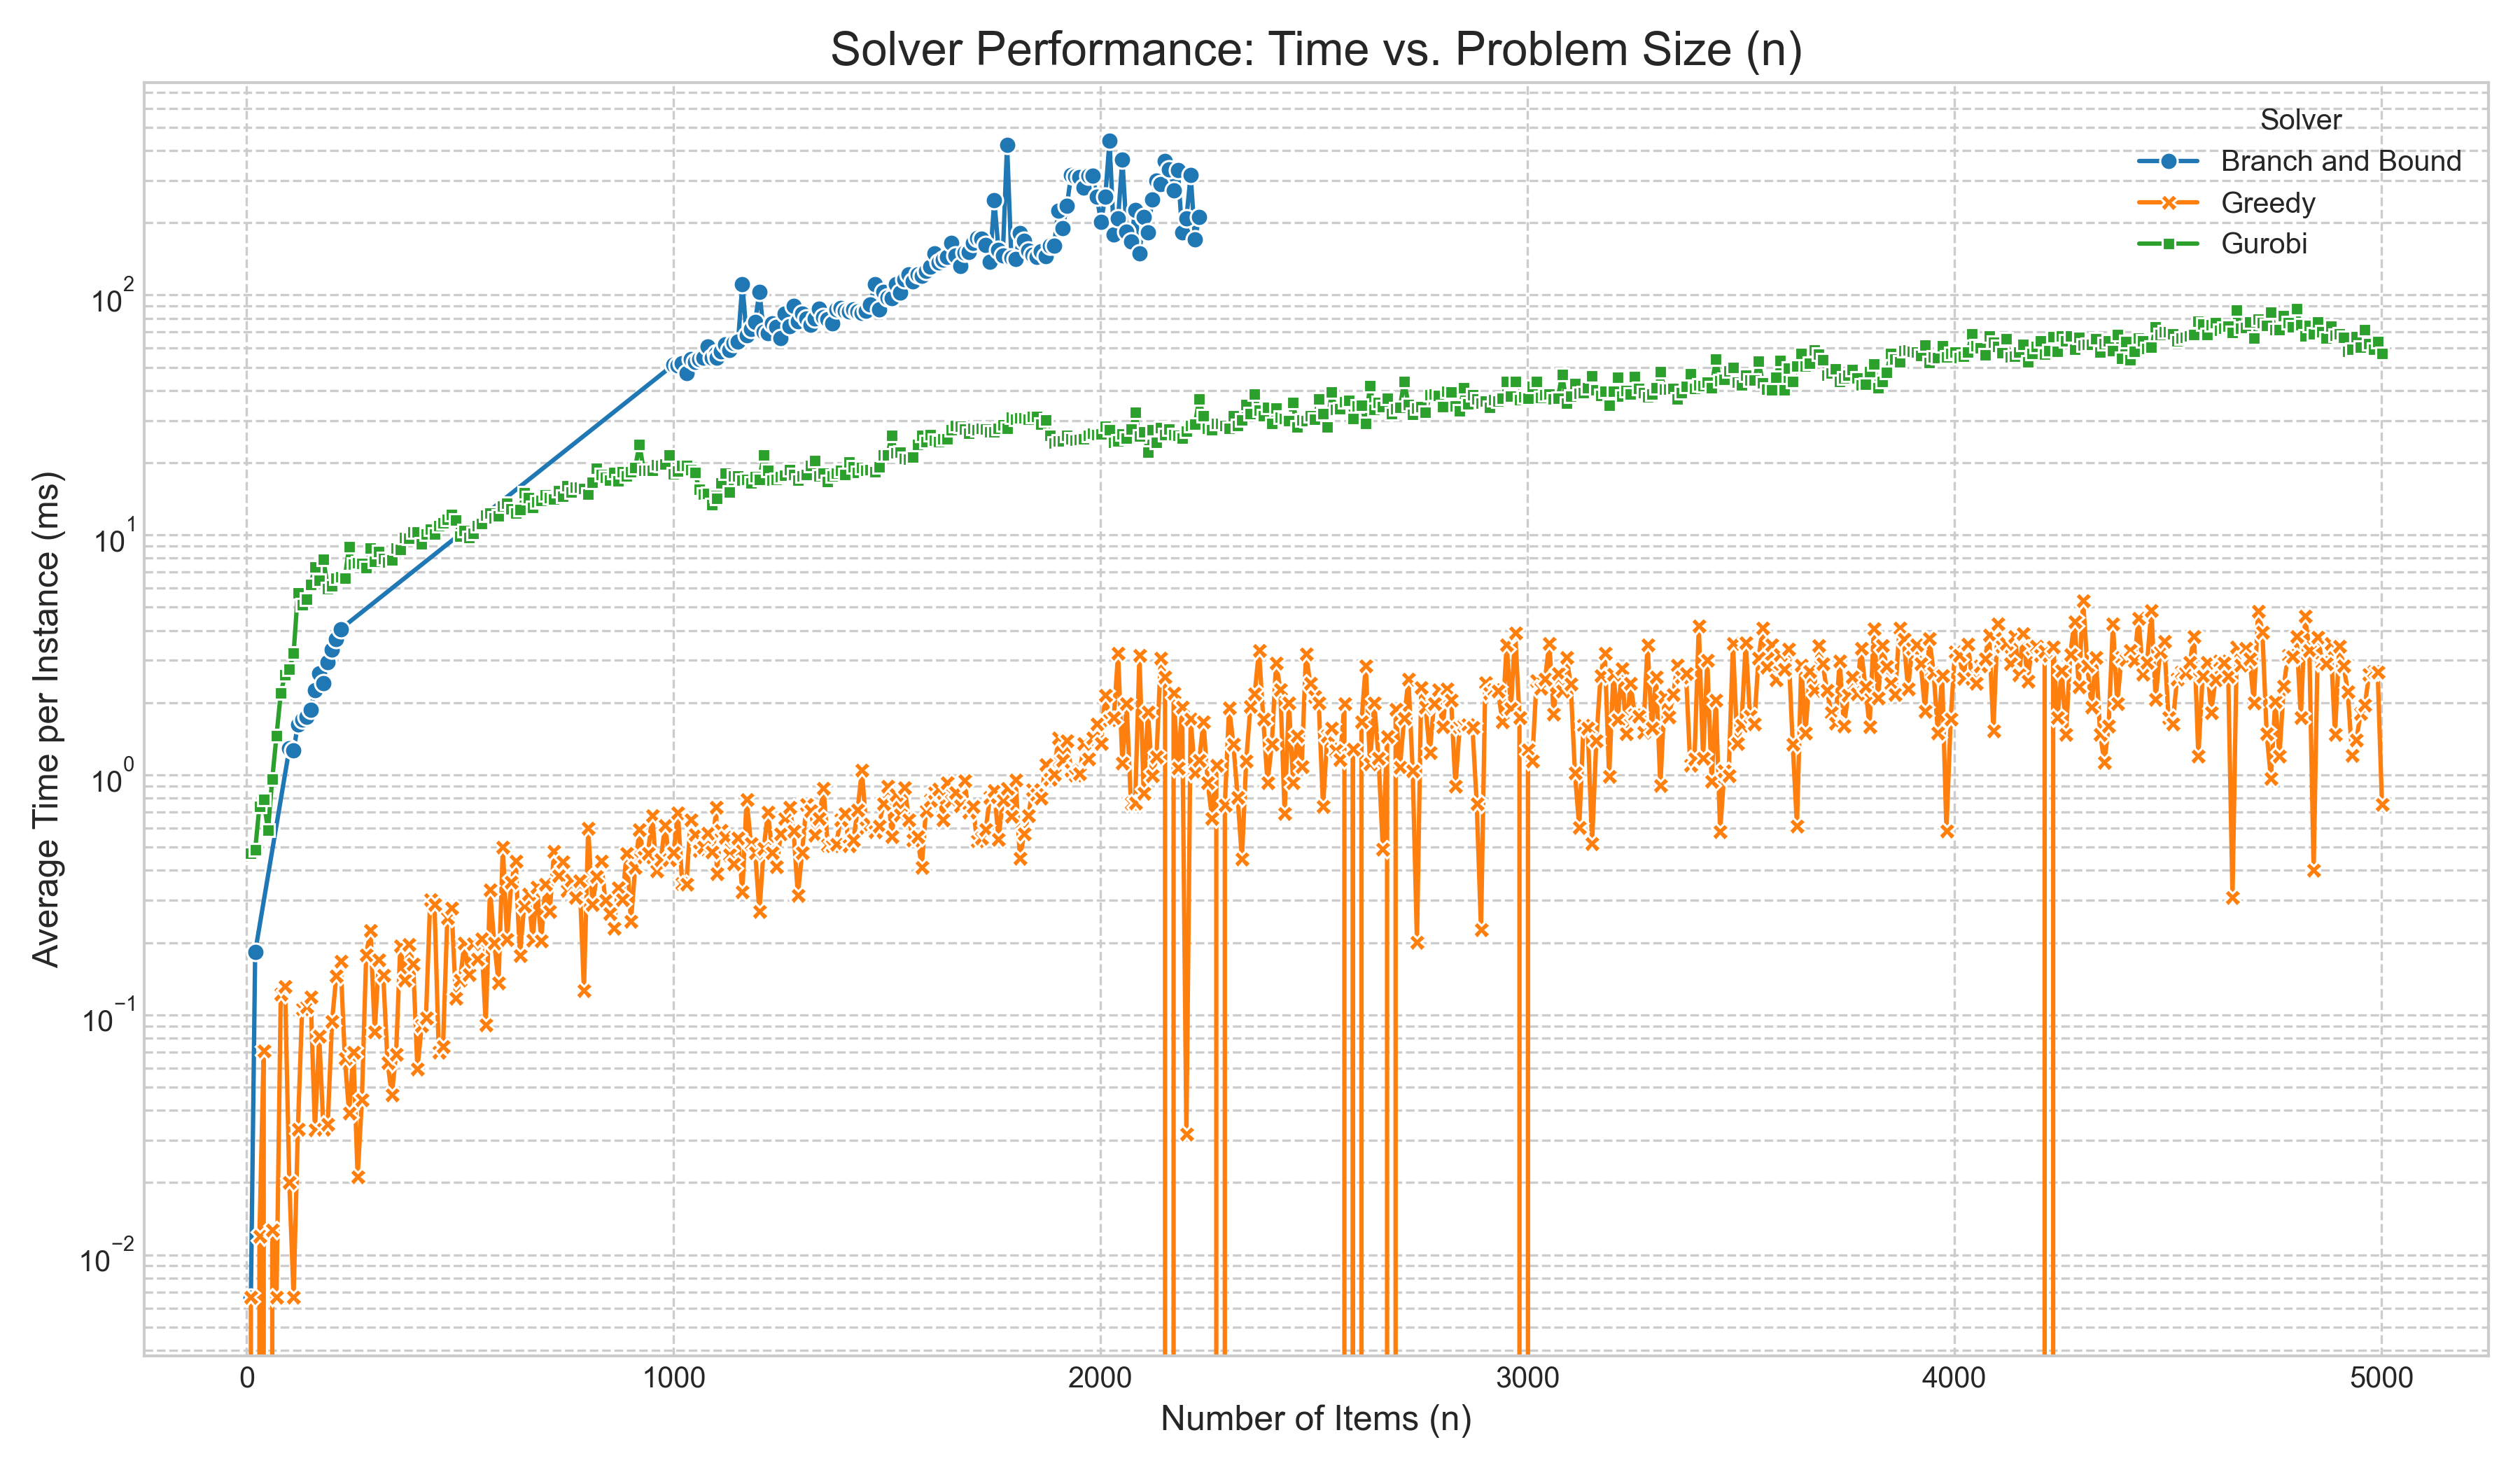
\includegraphics[width=\textwidth]{memory-explosion.png} 
                    \caption{Performance degradation due to memory constraints.}
                \end{figure}
                \vspace{-1.2em}
                \begin{itemize}
                    \item Suffer from the "curse of dimensionality".
                    \item Leads to a \textbf{memory explosion}, making them infeasible for large-scale problems.
                \end{itemize}
            \end{block}
        \end{column}

        % --- RIGHT COLUMN: Commercial Solvers ---
        \begin{column}{0.5\textwidth}
            \begin{block}{2. Time Complexity}
                \begin{figure}
                    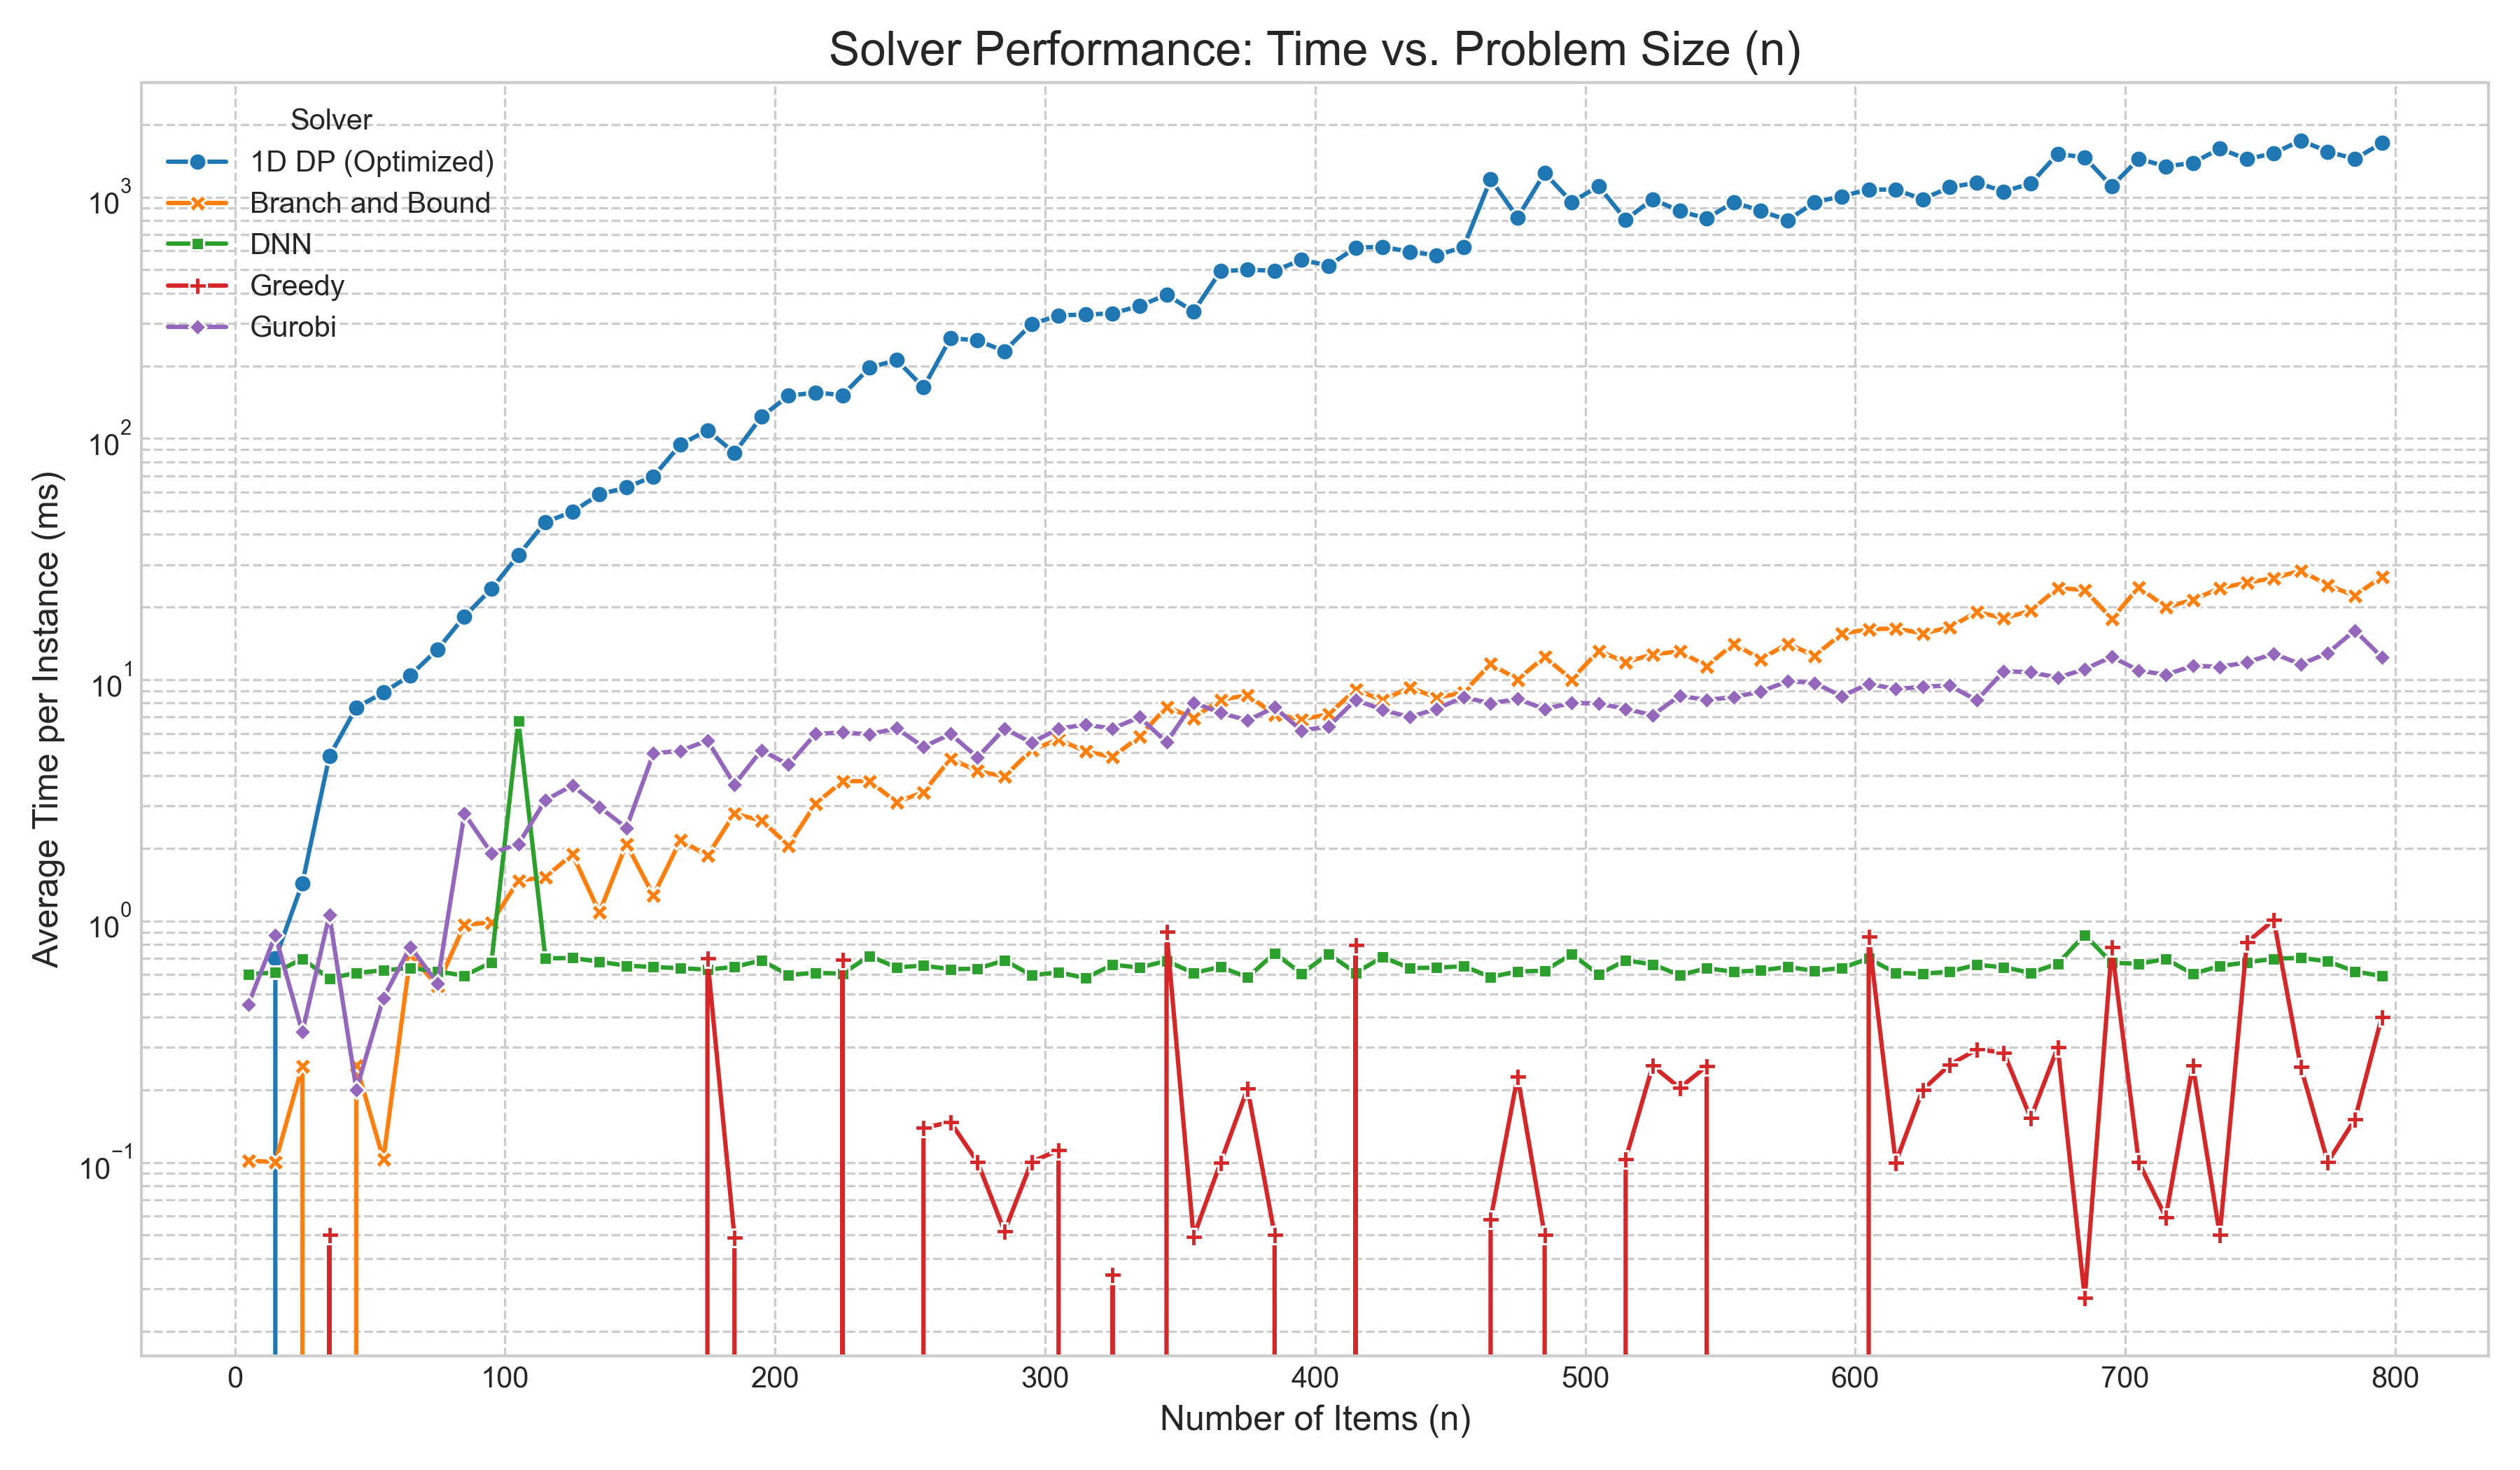
\includegraphics[width=\textwidth]{time-growth.png}
                    \caption{Performance comparison of various solvers.}
                \end{figure}
                \vspace{-1.2em}
                \begin{itemize}
                    \item Runtime of Commercial Solver like Gurobi still exhibits \textbf{exponential growth}, becoming a bottleneck for very large problems.
                \end{itemize}
            \end{block}
        \end{column}

    \end{columns}
\end{frame}

% --- SLIDE 2: RL Fundamentals & Bellman Equation ---
\begin{frame}
    \frametitle{RL Fundamentals \& The Bellman Equation}

    \begin{columns}[T]
        
        % --- LEFT COLUMN: RL Components for the 0/1 Knapsack Problem ---
        \begin{column}{0.5\textwidth}
            \begin{block}{Key RL Components for 0/1 KP}
                \begin{itemize}
                    \item \textbf{State ($s_t$):} The set of available items and the current remaining knapsack capacity. \vspace{0.5em}
                    
                    \item \textbf{Action ($a_t$):} The selection of one item from the available set that fits the capacity. \vspace{0.5em}
                    
                    \item \textbf{Policy ($\pi_\theta(a|s)$):} A neural network that maps the current state to a probability distribution over valid actions (items to select). \vspace{0.5em}
                    
                    \item \textbf{Reward ($R_{t+1}$):} The value ($v_i$) of the selected item. \vspace{0.5em}
                    
                    \item \textbf{Episode ($\tau$):} A sequence of item selections, ending when no more items can be legally packed.
                \end{itemize}
            \end{block}
        \end{column}
        
        % --- RIGHT COLUMN: Two Forms of the Bellman Equation ---
        \begin{column}{0.5\textwidth}
            
            \begin{alertblock}{1. Bellman Expectation Equation (Policy-based)}
                Calculates the value function $\mathbf{v}^\pi$ for a \textbf{given policy $\pi$}.
                \begin{align*}
                    \mathbf{v}^{\pi} = \mathbf{r}^{\pi} + \gamma \mathbf{P}^{\pi} \mathbf{v}^{\pi}
                \end{align*}
                This is the foundation for the \textbf{Critic} in Actor-Critic methods like PPO, which evaluates the current policy.
            \end{alertblock}
            
            \vspace{1em}

            \begin{block}{2. Bellman Optimality Equation (Value-based)}
                Defines the optimal value function $\mathbf{v}^*$ by finding the best action at each state.
                \begin{align*}
                    \mathbf{v}^{*} = \max_{a} \left( \mathbf{r}(a) + \gamma \mathbf{P}(a) \mathbf{v}^{*} \right)
                \end{align*}
                This is the target for value-based methods like Q-Learning, which directly learn the optimal policy.
            \end{block}

        \end{column}

    \end{columns}
\end{frame}

% --- Slide 3: REINFORCE Algorithm and Architecture ---
\begin{frame}
    \frametitle{REINFORCE: Algorithm and Architecture}

    \begin{columns}[T]
        
        % --- LEFT COLUMN: Algorithm Flowchart ---
        \begin{column}{0.5\textwidth}
            \begin{block}{Training Algorithm}
                \begin{figure}
                    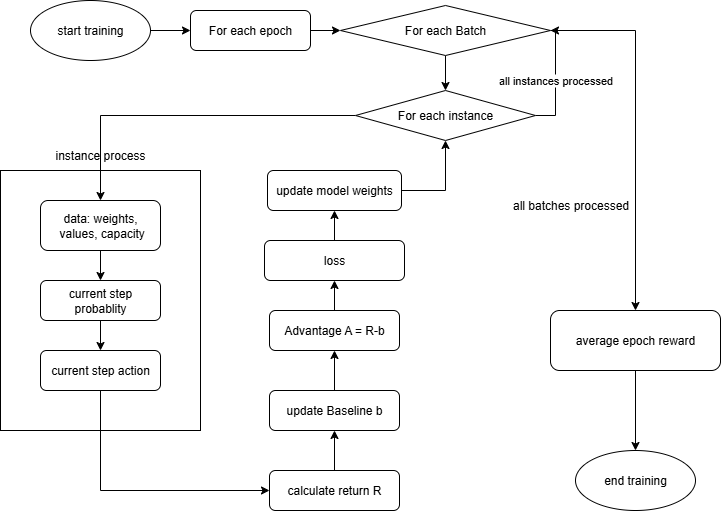
\includegraphics[width=\textwidth]{reinforce_training_manual.png}
                    \caption{The REINFORCE training loop with an EMA baseline.}
                \end{figure}

                \vspace{-1.5em}

                \begin{itemize}
                    % \item An entire episode (trajectory) is sampled per update.
                    \item The policy is updated based on the total return of the episode.
                    \item A baseline is used to reduce gradient variance.
                \end{itemize}
            \end{block}
        \end{column}

        % --- RIGHT COLUMN: Model Architecture ---
        \begin{column}{0.5\textwidth}
            \begin{block}{Model Architecture}
                \begin{figure}
                    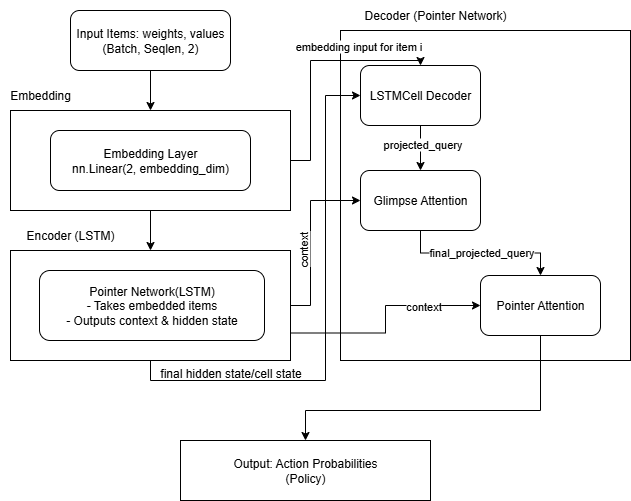
\includegraphics[width=\textwidth]{ptrn_arch.png}
                    \caption{Pointer Network-based architecture for sequential item selection.}
                \end{figure}
                \vspace{-1.5em}
                \begin{itemize}
                    \item One Actor and no Critic.
                \end{itemize}
            \end{block}
        \end{column}

    \end{columns}
\end{frame}

% --- Slide 4: PPO Algorithm and Model Architecture ---
\begin{frame}
    \frametitle{PPO: Algorithm and Architecture}

    \begin{columns}[T]
        \vspace{-1em}
        
        % --- LEFT COLUMN: PPO Algorithm Flowchart ---
        \begin{column}{0.5\textwidth}
            \begin{block}{Training Algorithm}
                \begin{figure}
                    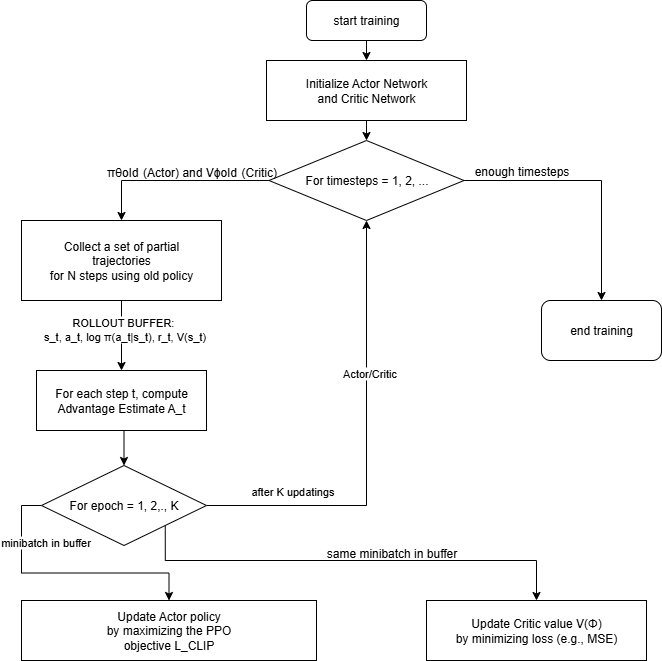
\includegraphics[width=0.85\textwidth, height=0.63\textheight]{PPO_training_manual.png}
                    \caption{The PPO training loop using an Actor-Critic framework.}
                \end{figure}
                \vspace{-1.5em}
                \begin{itemize}
                    \item Multiple optimization on the same minibatch.
                \end{itemize}
            \end{block}
        \end{column}

        % --- RIGHT COLUMN: PPO Model Architecture ---
        \begin{column}{0.5\textwidth}
            \begin{block}{Model Architecture}
                \begin{figure}
                    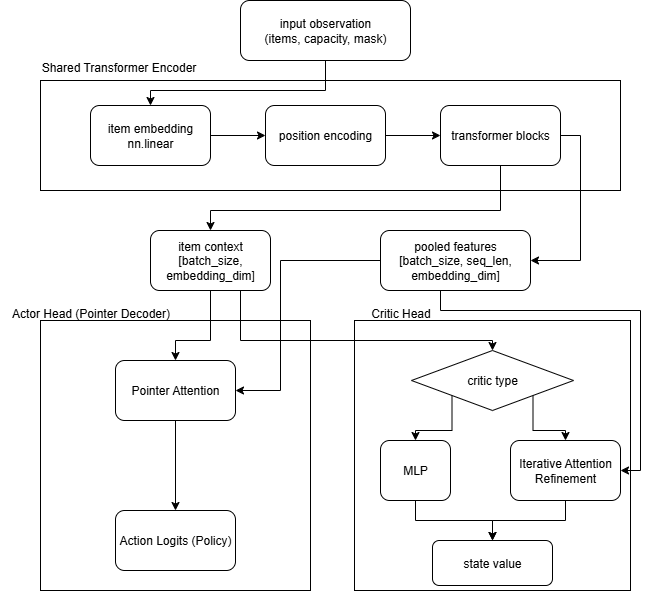
\includegraphics[width=0.85\textwidth, height=0.6\textheight]{ppo_model_manual.png}
                    \caption{The model has two heads: one for the policy (Actor) and one for the value (Critic).}
                \end{figure}
                \vspace{-1.5em}
                \begin{itemize}
                    \item Actor and Critic share the same encoder.
                    % \item The Actor outputs a probability distribution over actions (items).
                    % \item The Critic outputs a value estimate for the current state.
                \end{itemize}
            \end{block}
        \end{column}

    \end{columns}
\end{frame}

% \begin{frame}
%     \frametitle{Algorithm Implementation: REINFORCE with Baseline}
    
%     % The algorithmic environment is for typesetting pseudocode
%     % The [1] adds line numbers
%     \begin{algorithmic}[1]
%         \State \textbf{Initialize:} Policy network $\pi_\theta$, optimizer, and EMA baseline $b \gets 0$.
%         \vspace{0.5em}
        
%         \For{each epoch}
%             \For{each batch of problems}
%                 \State // \textit{1. Rollout Phase}
%                 \State Sample trajectories $\{\tau_1, \tau_2, ...\}$ using the current policy $\pi_\theta$.
%                 \vspace{0.5em}
                
%                 \State // \textit{2. Advantage Calculation}
%                 \State Compute returns $R(\tau_i)$ for each trajectory (total packed value).
%                 \State Update EMA baseline: $b \gets \beta \cdot b + (1-\beta) \cdot \text{mean}(R)$.
%                 \State Calculate advantage for each trajectory: $\hat{A}(\tau_i) \gets R(\tau_i) - b$.
%                 \vspace{0.5em}
                
%                 \State // \textit{3. Policy Update}
%                 \State Calculate policy loss: $\mathcal{L}(\theta) \gets - \frac{1}{N}\sum_{i} \log p_\theta(\tau_i) \cdot \hat{A}(\tau_i)$.
%                 \State Update policy network parameters $\theta$ via backpropagation.
%             \EndFor
%         \EndFor
%     \end{algorithmic}
    
%     \vfill % Pushes the block to the bottom
    
%     \begin{alertblock}{Key Idea}
%         An Exponential Moving Average (EMA) baseline ($b$) is subtracted from the return ($R$) to calculate the \textbf{advantage} ($\hat{A}$). This significantly reduces the variance of the policy gradient, leading to more stable and faster training.
%     \end{alertblock}

% \end{frame}

% % --- Slide 2: Choosing the Right Reinforcement Learning Approach ---
% \begin{frame}
%     \frametitle{Choosing the Right Reinforcement Learning Approach}

%     \begin{columns}[T]
        
%         % --- LEFT COLUMN: Policy-based vs. Value-based ---
%         \begin{column}{0.5\textwidth}
%             \begin{block}{Value-based Methods (e.g., DQN)}
%                 \begin{itemize}
%                     \item \textbf{What it learns:} A value function $Q(s, a)$ that estimates the max future reward.
%                     \item \textbf{How it acts:} Chooses the action with the highest estimated value.
%                     \item \textbf{Limitation:} Can be inefficient or unstable in large/continuous action spaces, as is the case for KP with many items.
%                 \end{itemize}
%             \end{block}

%             \begin{alertblock}{Policy-based Methods (Our Choice)}
%                 \begin{itemize}
%                     \item \textbf{What it learns:} Directly learns a policy $\pi(a|s)$, a probability distribution over actions.
%                     \item \textbf{How it acts:} Samples an action directly from the policy.
%                     \item \textbf{Advantage:} More effective for complex action spaces and can learn stochastic policies, which aids exploration.
%                 \end{itemize}
%             \end{alertblock}
%         \end{column}

%         % --- RIGHT COLUMN: MC vs. TD updates ---
%         \begin{column}{0.5\textwidth}
%             \begin{block}{Monte Carlo Updates (e.g., REINFORCE)}
%                 \begin{itemize}
%                     \item \textbf{How it updates:} Waits until an entire episode is finished, then updates the policy based on the final total reward.
%                     \item \textbf{Limitation:} High variance in updates because one good/bad final outcome is attributed to all actions taken, leading to unstable training.
%                 \end{itemize}
%             \end{block}
            
%             \begin{alertblock}{Temporal Difference (TD) Updates (PPO's basis)}
%                 \begin{itemize}
%                     \item \textbf{How it updates:} Updates the policy after each step (or a few steps), using a learned value estimate (from a Critic) to judge actions.
%                     \item \textbf{Advantage:} Lower variance and more sample-efficient as it learns from every step. PPO further improves stability with its clipped objective.
%                 \end{itemize}
%             \end{alertblock}
%         \end{column}

%     \end{columns}

%     \vfill % Pushes the summary to the bottom
%     \small\textit{Conclusion: Our framework uses PPO, a policy-based, Actor-Critic (TD) method, to leverage its stability and effectiveness in large action spaces.}
    
% \end{frame}

% % --- Slide 3: Policy Gradient Algorithm Formulas ---
% \begin{frame}
%     \frametitle{Policy Gradient Algorithms: REINFORCE vs. PPO}

%     \begin{columns}[T]
        
%         % --- LEFT COLUMN: REINFORCE ---
%         \begin{column}{0.5\textwidth}
%             \begin{block}{REINFORCE (Monte Carlo)}
%                 \textbf{Objective:} Maximize the expected total reward.
%                 \begin{align*}
%                     J(\theta) = \mathbb{E}_{\tau \sim \pi_\theta}[R(\tau)]
%                 \end{align*}
                
%                 \textbf{Policy Gradient:} The policy is updated using the gradient of the objective. The update rule relies on the full return $G_t$.
%                 \begin{align*}
%                      \nabla_\theta J(\theta) \propto \sum_{t=0}^{T} \nabla_\theta \log \pi_\theta(a_t|s_t) G_t 
%                 \end{align*}
                
%                 \textbf{Where:}
%                 \begin{itemize}
%                     \item $\pi_\theta(a_t|s_t)$ is the policy network.
%                     \item $G_t = \sum_{k=t}^{T} \gamma^{k-t} r_k$ is the total discounted reward from step $t$.
%                 \end{itemize}
%                 \textbf{Limitation:} High variance due to using the noisy full return $G_t$.
%             \end{block}
%         \end{column}

%         % --- RIGHT COLUMN: PPO ---
%         \begin{column}{0.5\textwidth}
%             \begin{alertblock}{PPO (Temporal Difference)}
%                 \textbf{Objective (Clipped Surrogate):} PPO constrains the policy change to improve stability.
%                 \begin{align*}
%                     L^{CLIP}(\theta) = \hat{\mathbb{E}}_t \Big[ \min \big( r_t(\theta)\hat{A}_t, \\ 
%                     \text{clip}(r_t(\theta), 1-\epsilon, 1+\epsilon) \hat{A}_t \big) \Big]
%                 \end{align*}
                
%                 \textbf{Where:}
%                 \begin{itemize}
%                     \item $r_t(\theta) = \frac{\pi_\theta(a_t|s_t)}{\pi_{\theta_{old}}(a_t|s_t)}$ is the probability ratio.
%                     \item $\hat{A}_t = G_t - V(s_t)$ is the \textbf{Advantage Estimate}, which has lower variance than $G_t$.
%                     \item $\epsilon$ is a hyperparameter for clipping.
%                 \end{itemize}
%                 \textbf{Advantage:} Stable, reliable, and sample-efficient.
%             \end{alertblock}
%         \end{column}

%     \end{columns}
% \end{frame}

% --- Subsection 3.2: Model Architecture ---
% \subsection{Model Architecture}

% % --- Slide 4: Overall Framework ---
% \begin{frame}
%     \frametitle{Our Proposed End-to-End RL Framework}
    
%     \begin{figure}
%         % --- Placeholder for your overall framework diagram ---
%         % --- e.g., a flowchart showing State -> Model -> Action -> Reward -> Update ---
%         \includegraphics[width=\textwidth]{placeholder.png}
%         \caption{The end-to-end process of solving a Knapsack instance using our PPO-based framework.}
%     \end{figure}

%     \begin{itemize}
%         \item Our framework takes a raw knapsack instance as input.
%         \item The \textbf{Actor-Critic} model outputs a policy for item selection.
%         \item The agent builds the solution sequentially.
%         \item The policy is updated using the \textbf{Proximal Policy Optimization (PPO)} algorithm.
%     \end{itemize}
% \end{frame}

% % --- Slide 5: Detailed Neural Network Architecture ---
% \begin{frame}
%     \frametitle{Detailed Model Architecture}
    
%     \begin{figure}
%         % --- Placeholder for your detailed neural network diagram ---
%         % --- e.g., showing input embeddings, CNN layers, attention, output heads ---
%         \includegraphics[width=\textwidth]{placeholder.png}
%         \caption{The internal architecture of our policy and value networks.}
%     \end{figure}

%     % --- You can use columns to describe different parts of the architecture ---
%     \begin{columns}[T]
%         \begin{column}{0.5\textwidth}
%             \textbf{Encoder:}
%             \begin{itemize}
%                 \item Processes the set of items.
%                 \item Captures relationships between items.
%             \end{itemize}
%         \end{column}
%         \begin{column}{0.5\textwidth}
%             \textbf{Decoder (Actor-Critic):}
%             \begin{itemize}
%                 \item Selects items sequentially.
%                 \item Outputs the action probability (policy) and state value.
%             \end{itemize}
%         \end{column}
%     \end{columns}
% \end{frame}